%\documentclass[10pt]{letter}
%\usepackage[utf8]{inputenc}

%%%%%%%%%%%%%%%%%%%%%%%%%%%%%%%%%%%%%%%%%%%%%%%%%
% compile with LuaLatex
%%%%%%%%%%%%%%%%%%%%%%%%%%%%%%%%%%%%%%%%%%%%%%%%%%%%%%%
\documentclass[11pt]{report}
\usepackage{epsfig}
\usepackage{amssymb,amsmath,amsfonts}
\usepackage[activeacute,american]{babel}
%\usepackage[utf8]{inputenc}
\usepackage{subfiles}
\usepackage{cite}
\usepackage{csquotes}
\usepackage{esvect}
\usepackage[acronym,nonumberlist]{glossaries}
\renewcommand{\acronymname}{Nomenclature}
\usepackage{multicol}
\usepackage{caption} 
\usepackage{float}
\usepackage[
    math-style=ISO,      % Upper Case Greek is in italics
    bold-style=ISO,      % Bold math is in italics
    partial=upright,     % nabla and partial upright
    nabla=upright,
  ]{unicode-math}
\topmargin 1.2cm 
\textwidth 16.1cm
\textheight 22.5cm
\oddsidemargin 0.7cm
\setcounter{tocdepth}{5}
\addtolength{\voffset}{-2.4cm}
\addtolength{\hoffset}{-0.5cm}

\usepackage{setspace}
%\doublespacing
\onehalfspacing
\usepackage{caption}
 \captionsetup[figure]{labelfont={bf},name={Figura},labelsep=period}


%%%%%%%%%%%%%%%%%%%%%%%%%%%%%%% 
% citas
% \footnotetext{Mott, Robert L. Mecanica de Fluidos 6/e. Pearson educación, 2006.}
% \footnotetext{Pritchard, Philip J. Fox and McDonald’s Introduction to Fluid Mechanics (8th ed.). John Wiley $\&$ Sons. (2011).}
% \footnotetext{Munson, Bruce R., et al. "Fundamentals of Fluid Mechanics, John Wiley $\&$ Sons." Inc., USA (2006).}
%%%%%%%%%%%%%%%%%%%%%%%%%%%%%%% 

%%%%%%%%%%%%%%%%%%%%%%%%%%%%%%%%%
\begin{document}
\centering{ \textbf{\Large{Mec\'anica de fluidos}}}

\centering {\Large{2$^\circ$ semestre 2020: 541209-1}}
\vspace{1cm}

\flushleft{ \large \underline{\textbf{Pr\'actica 6: Aplicaci\'on y selecci\'on de bombas}}}

%%%%%%%%%%%%%%%%%%%%%%%%%
\vspace{1cm}

\underline {Problema 1 (Adaptado del P. 10.68 Fox\footnote{footnotes working fine}):}
\vspace{0.2cm}

La bomba presentada en el sistema de la figura~\ref{fig:fig1} extrae agua de un sumidero y la env\'ia a un tanque abierto a trav\'es de $400$\,m de tuber\'ia de acero de $4$ pulgadas, c\'edula 40. La tuber\'ia de la linea de succi\'on vertical tiene una longitud de $2$\,m e incluye una v\'alvula de pie tipo disco de v\'astago y un codo est\'andar de $90^\circ$. La linea de descarga incluye dos codos est\'andar de $90^\circ$, una v\'alvula de verificaci\'on tipo giratioria y una v\'alvula de compuerta. El flujo volum\'etrico de diseño corresponde a $800$\,L/min. 
\renewcommand{\theenumi}{\Alph{enumi}}
\begin{enumerate}
\item Determine el $NPSH_A$ para el sistema.
\item Seleccione una bomba adecuada para este sistema.
\item Para la bomba seleccionada, determine la condici\'on de operaci\'on
%\item Suponga que la v\'alvula de compuerta es cerrada, hasta quedar $1/4$ abierta. Calc\'ule el flujo volum\'etrico y la carga elevada por la bomba para esta condici\'on
\end{enumerate}


\begin{figure}[H]
\centering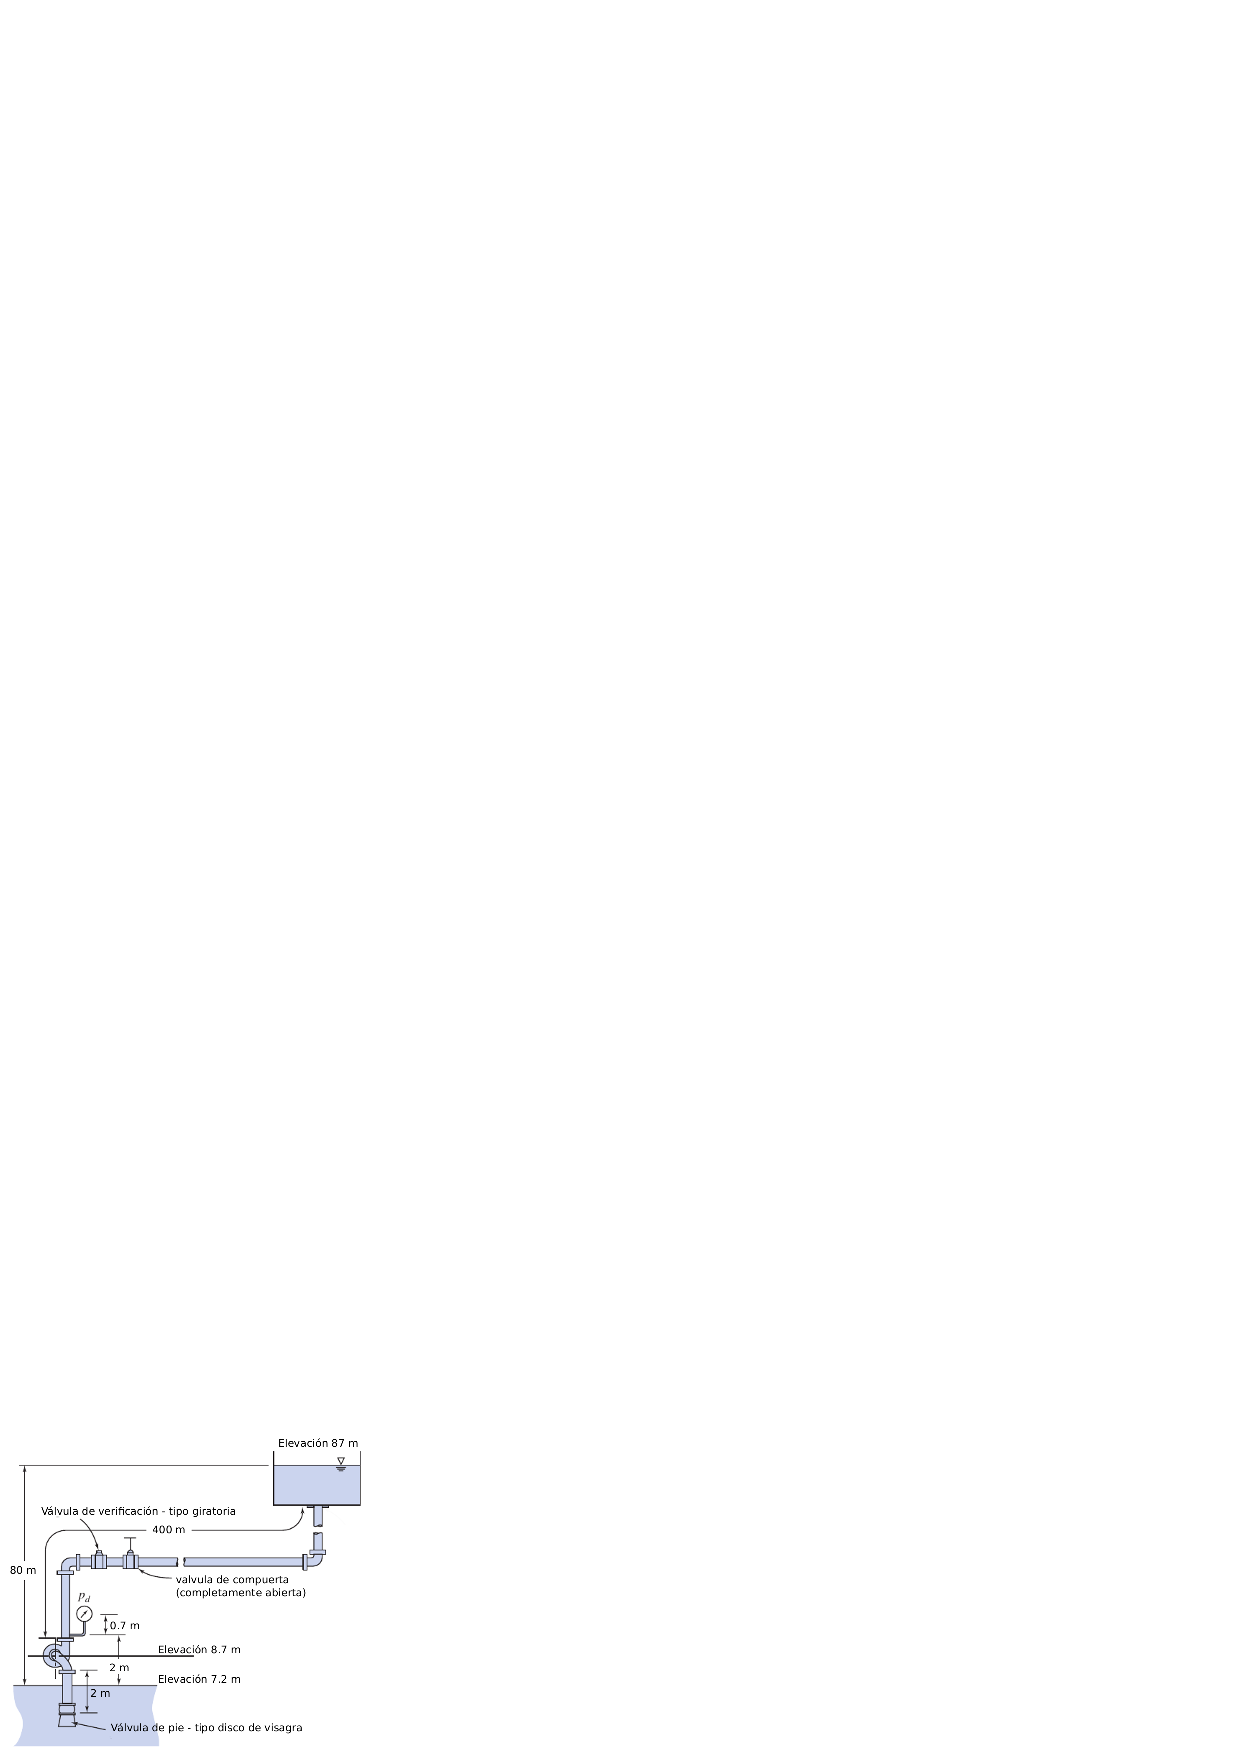
\includegraphics[width=0.5\textwidth]{Figures/p1.png}
\caption{\label{fig:fig1} }
\end{figure}



 \footnotetext{Pritchard, Philip J. Fox and McDonald’s Introduction to Fluid Mechanics (8th ed.). John Wiley $\&$ Sons. (2011).}





%%%%%%%%%%%%%%%%%%%%%%%%%
%%%%%%%%%%%%%%%%%%%%%%%%%
\end{document}
